\documentclass[conference]{IEEEtran}
\IEEEoverridecommandlockouts

\usepackage{cite}
\usepackage{amsmath,amssymb,amsfonts}
\usepackage{graphicx}
\usepackage{textcomp}
\usepackage[table]{xcolor}
\usepackage{array}
\usepackage{booktabs}
\usepackage{url}
\usepackage{float}
\usepackage{placeins}
\usepackage{tikz}
\usetikzlibrary{arrows.meta,positioning,calc}
\usepackage{pgfplots}
\usepgfplotslibrary{groupplots}
\pgfplotsset{compat=1.18}

\graphicspath{{figures/}}

\begin{document}

\renewcommand{\topfraction}{0.9}
\renewcommand{\bottomfraction}{0.8}
\renewcommand{\textfraction}{0.07}
\renewcommand{\floatpagefraction}{0.7}
\setcounter{topnumber}{4}
\setcounter{bottomnumber}{4}
\setcounter{totalnumber}{6}

\title{Model Compression and Input Optimization Co-Design for Edge Driver Monitoring Systems}

\author{
  \IEEEauthorblockN{1\textsuperscript{st} Oumar Mamoun Ibrahim}
  \IEEEauthorblockA{\textit{Department of Computer Engineering} \\
  \textit{University of Sharjah} \\
  Sharjah, UAE \\
  U22200741@sharjah.ac.ae}
  \and
  \IEEEauthorblockN{2\textsuperscript{nd} Mohamad Khairi bin Ishak}
  \IEEEauthorblockA{\textit{Department of Computer Engineering} \\
  \textit{University of Sharjah} \\
  Sharjah, UAE \\
  mishak@sharjah.ac.ae}
  \and
  \IEEEauthorblockN{3\textsuperscript{rd} Ahmed Atef Abouelhamd}
  \IEEEauthorblockA{\textit{Department of Computer Engineering} \\
 \textit{University of Sharjah} \\
 Sharjah, UAE \\
 U23104122@sharjah.ac.ae}
}

\maketitle

\begin{abstract}
Edge driver monitoring systems (DMS) must detect distraction and drowsiness in real time on small compute and memory budgets. We study whether model compression and input preprocessing can be co-designed for this task without violating a safety recall floor. On the Driver Monitoring Dataset with a subject-disjoint split, we combine structured $\ell_1$-norm channel pruning and 8-bit integer (INT8) quantization on YOLO11n and YOLO26n with three input methods (resize, static crop, and overlapping collage) from 640 to 80 pixels, and we score every configuration by macro-recall on the same frames and boxes over three seeds. YOLO11n holds the 5-point recall floor up to 70\% sparsity, and quantization-aware training (QAT) brings this model to 1.29~MB at 84.8\% macro-recall against 86.4\% for the baseline. The overlapping collage gives the highest recall at every resolution down to 160 pixels. The cheapest configuration that holds the floor is the 160-pixel collage with 30\% sparsity and INT8 post-training quantization (PTQ), which needs $24.5\times$ less compute and $4.8\times$ less storage but passes only narrowly. The 320-pixel collage with INT8 gives the highest recall, 92.9\%, at $4.0\times$ less compute. Heavier pruning at reduced input did not transfer from validation to test drivers.
\end{abstract}

\begin{IEEEkeywords}
Object Detection, Driver Monitoring Systems, Edge Deployment, Model Pruning, Quantization
\end{IEEEkeywords}


\section{Introduction}
Most computer vision models are designed for high-performance systems, which increases neural network size and the computation and storage required for inference~\cite{b1}. This makes direct deployment on edge devices impractical~\cite{b2,b3}. To bridge this gap, practitioners adapt models to constrained hardware through pruning~\cite{b4}, quantization~\cite{b5}, and knowledge distillation~\cite{b6}. These methods reduce parameter count and inference cost from different angles. Edge-deployed driver monitoring systems (DMS) are particularly demanding, because the detector must evaluate every frame in real time to catch distraction and drowsiness cues.

This work addresses one research question:
\begin{itemize}
    \item How do model-level compression and input-level preprocessing compare in isolation, and can their co-design reduce edge cost without violating a safety recall limit?
\end{itemize}

We approach the question from the model side and the input side, then combine both in one co-designed pipeline. On the model side, we evaluate structured $\ell_1$-norm channel pruning, which removes the weakest convolutional channels~\cite{b9}. Structured pruning reduces floating-point operations (FLOPs) on commodity hardware and needs no sparse accelerator. We also evaluate post-training quantization (PTQ) and quantization-aware training (QAT), which convert 32-bit floating-point (FP32) networks to 8-bit integers (INT8). On the input side, we evaluate a static $400\times400$ region of interest (RoI) crop and a static overlapping collage across input resolutions of 640, 320, 160, and 80 pixels.

The main contributions of this paper are:
\begin{itemize}
    \item A model-input co-design framework that searches input method, resolution, sparsity, and quantization together under one macro-recall floor, using validation data only.
    \item An evaluation protocol that scores every configuration on the same frames and ground-truth boxes at one threshold, so an object removed by the input step counts as a missed detection.
    \item A multi-seed study of $\ell_1$-norm pruning, INT8 PTQ, and true fake-quantized QAT on YOLO11n and YOLO26n, with clip-level confidence intervals for the small test set.
    \item A measured account of why INT8 detection recall becomes unstable when the output layers of the detection head are quantized, and how keeping them in floating point removes the instability.
\end{itemize}
The code, configurations, and per-run results that reproduce every table and figure are available at \url{https://github.com/IamOumarIbrahim/pruning-missed-detection}.


\begin{table}[t]
\caption{Coverage of prior work versus this paper}
\label{tab:gap}
\centering
\footnotesize
\setlength{\tabcolsep}{3pt}
\begin{tabular}{@{}lccccc@{}}
\toprule
\textbf{Work} & \textbf{Pruning} & \textbf{Quant.} & \textbf{RoI} & \textbf{DMS} & \textbf{Joint} \\
\midrule
Filter/channel pruning \cite{b9,b10,b11,b12} & $\checkmark$ & -- & -- & -- & -- \\
Deep compression \cite{b8}                   & $\checkmark$ & $\checkmark$ & -- & -- & -- \\
Quantization \cite{b13,b14}                  & -- & $\checkmark$ & -- & -- & -- \\
Tiling / multi-scale RoI \cite{b18,b19}      & -- & -- & $\checkmark$ & -- & -- \\
DMS / distraction \cite{b20,b21,b22}         & -- & -- & -- & $\checkmark$ & -- \\
\midrule
\textbf{This work} & $\checkmark$ & $\checkmark$ & $\checkmark$ & $\checkmark$ & $\checkmark$ \\
\bottomrule
\end{tabular}
\end{table}

\section{Related Work}

\subsection{Model Compression for Edge Object Detection}
Deploying detectors on embedded hardware relies on pruning, quantization, and efficient architecture design. Unstructured pruning removes individual low-magnitude weights~\cite{b8}, but the resulting sparsity seldom yields real speedups on commodity accelerators. Structured pruning removes entire filters or channels and produces a smaller dense network. Li \emph{et al.}~\cite{b9} rank filters by their $\ell_1$ norm. He \emph{et al.}~\cite{b10} select channels through LASSO regression with feature-map reconstruction. Liu \emph{et al.}~\cite{b11} exploit sparsity in batch-normalization scale factors. Fang \emph{et al.}~\cite{b12} extend structural pruning to arbitrary architectures through dependency graphs, which matters for YOLO models whose concatenations and residual links couple channels across layers.

Quantization lowers numerical precision to cut memory traffic and latency. Jacob \emph{et al.}~\cite{b13} introduced integer-arithmetic-only inference with QAT, and Krishnamoorthi~\cite{b14} compared PTQ and QAT for INT8 deployment. Han \emph{et al.}~\cite{b8} showed that pruning and quantization are complementary when applied jointly.

The YOLO family is a standard choice for real-time detection on constrained devices. YOLOv7 introduced trainable bag-of-freebies and planned re-parameterization~\cite{b15}. YOLOv10 removed non-maximum suppression (NMS) through consistent dual assignments~\cite{b16}. YOLO11 introduced C3k2 and C2PSA blocks~\cite{b17}. YOLO26 adds NMS-free inference by default and removes distribution focal loss~\cite{b26}. Compression studies of these detectors typically fix the input, compress the network, and report mean average precision (mAP) on general-purpose benchmarks. Recall on safety-critical minority classes receives far less attention.

\subsection{Input-Level and RoI Optimization}
Input resolution is a primary driver of inference cost, so cropping, tiling, and resolution selection are natural levers for real-time systems. Unel \emph{et al.}~\cite{b18} showed that tiling improves small-object detection. Najibi \emph{et al.}~\cite{b19} proposed AutoFocus, which processes only selected high-resolution regions. These methods target generic scenes in which object locations are unpredictable. In an in-cabin camera, the driver occupies a predictable region of the frame, which makes a static RoI a natural design choice.

\subsection{Driver Monitoring Systems}
Deep learning has become the standard approach to driver distraction and drowsiness detection. The Driver Monitoring Dataset (DMD)~\cite{b20} provides multi-modal in-cabin recordings with annotated attention and alertness states. Abouelnaga \emph{et al.}~\cite{b21} studied real-time distracted driver posture classification and treated inference speed as a design constraint. Kashevnik \emph{et al.}~\cite{b22} surveyed driver distraction detection methods and organized them into a common framework.

\subsection{Research Gap}
Existing work treats compression, input-level optimization, and driver monitoring largely in isolation (Table~\ref{tab:gap}). Three gaps stand out:
\begin{itemize}
    \item YOLO compression studies optimize mAP on general benchmarks. Recall on safety-critical minority classes receives little attention.
    \item Static RoI strategies have not been compared systematically across input resolutions for in-cabin behavior detection.
    \item No prior work has selected pruning, quantization, and input preprocessing jointly under a recall constraint for DMS.
\end{itemize}



\section{Methodology}

\subsection{Proposed Co-Design Framework}
\label{sec:framework}
Existing YOLO compression work fixes the input and compresses the network. Our framework differs in three ways. First, the input and the model are one search space: a configuration $c$ is a tuple of input method, resolution, sparsity, and quantization. Second, the input comes first. Each model is trained on the input it will see, and pruning starts from that checkpoint, not from a full-frame model. Third, input loss and model loss share one denominator: every configuration is scored on the same frames and boxes, so an object the crop removes is a miss.

The study has three phases. Phase~I measures pruning and quantization alone. Phase~II measures input methods alone. Phase~III searches their combinations and selects the cheapest configuration that holds the recall floor on validation data:
\begin{equation}
\label{eq:selection}
c^{*} = \arg\min_{c}\ \mathrm{GFLOPs}(c)
\quad \text{s.t.} \quad
R^{\text{val}}(c) \geq R^{\text{val}}_{\text{base}} - \delta,
\end{equation}
where $R^{\text{val}}$ is validation macro-recall, $R^{\text{val}}_{\text{base}}$ is that of the FP32 baseline, and $\delta=0.05$ is the safety margin defined in (\ref{eq:floor}).

\subsection{Models and Dataset}
\label{sec:data}
YOLO11n has 2.59M parameters and 6.50~GFLOPs at $640\times640$ and integrates C3k2 blocks with C2PSA spatial attention. Phase~I also evaluates YOLO26n, with 2.51M parameters and 5.90~GFLOPs, which is NMS-free and has no distribution focal loss. DMD contains $1280\times720$ RGB in-cabin video of drivers performing drowsy and distracted behaviors. We extract 15{,}723 frames at 1~FPS from 14 subjects and center-crop them to $640\times640$. Two annotators labeled each frame. Negative frames have no box. Positive frames have one box from four classes: yawning, hand-over-mouth, drinking, or phone use. Negative frames form $\approx81\%$ of all frames (12{,}722), and phone use forms $\approx81\%$ of positive frames (2{,}437).

Subjects are split 8:3:3 so that no driver appears in two splits. This tests generalization to new drivers, which random frame splits cannot do because consecutive frames of one driver are nearly identical. Table~\ref{tab:splits} gives the composition of each split and how it is used. Training subjects fit all weights, including fine-tuning after pruning, QAT, and PTQ range calibration. Validation subjects select the best checkpoint of each run and the final configuration in (\ref{eq:selection}). Test subjects are used once, for the reported numbers.

\begin{table}[t]
\caption{Subject-disjoint splits and their use}
\label{tab:splits}
\centering
\footnotesize
\setlength{\tabcolsep}{2.5pt}
\begin{tabular}{@{}lrrr@{}}
\toprule
 & \textbf{Train} & \textbf{Validation} & \textbf{Test} \\
\midrule
Subjects & 8 & 3 & 3 \\
Subject IDs & 1, 4, 6--9, 13, 14 & 2, 3, 11 & 5, 10, 12 \\
Frames & 9{,}087 & 3{,}423 & 3{,}213 \\
Clips & 40 & 15 & 13 \\
Yawning frames (clips) & 94 (10) & 32 (5) & 33 (5) \\
Hand-over-mouth frames (clips) & 83 (10) & 30 (4) & 28 (5) \\
Drinking frames (clips) & 154 (8) & 54 (3) & 56 (3) \\
Phone-use frames (clips) & 1{,}417 (9) & 523 (3) & 497 (3) \\
\midrule
Weights, fine-tuning, QAT & \checkmark & -- & -- \\
PTQ calibration (300 frames) & \checkmark & -- & -- \\
Best checkpoint per run & -- & \checkmark & -- \\
Configuration selection & -- & \checkmark & -- \\
Reported results & -- & -- & \checkmark \\
\bottomrule
\end{tabular}
\end{table}

Baselines start from COCO-pretrained weights and train for 100 epochs in Ultralytics 8.4 on an NVIDIA RTX~4060 8\,GB GPU with batch size 16 and three seeds. The automatic optimizer setting resolves to MuSGD with learning rate 0.01, momentum 0.9, and weight decay 0.0005.

\subsection{Evaluation Protocol}
\label{sec:protocol}
All phases use one protocol. Detections are matched to ground truth greedily by confidence, within a class, at an intersection over union (IoU) of 0.5. All metrics use a fixed confidence threshold of $\tau=0.5$. A validation-tuned threshold is reported only as a sensitivity check. Precision $P_c$ and recall $R_c$ of class $c$ give the class score in (\ref{eq:f1}):
\begin{equation}
\label{eq:f1}
F1_c = \frac{2\,P_c\,R_c}{P_c + R_c}.
\end{equation}
Macro metrics in (\ref{eq:macro}) are unweighted means over the four classes:
\begin{equation}
\label{eq:macro}
R = \frac{1}{4}\sum_{c=1}^{4} R_c, \quad
P = \frac{1}{4}\sum_{c=1}^{4} P_c, \quad
F1 = \frac{1}{4}\sum_{c=1}^{4} F1_c.
\end{equation}
Macro-recall $R$ from (\ref{eq:macro}) is the primary safety metric, because automotive DMS guidance treats a missed distraction or drowsiness event as a hazard and a false alarm as an annoyance~\cite{euroncap2026driver,isots5283}. A configuration is safe if it holds the floor
\begin{equation}
\label{eq:floor}
R \geq R_{\text{floor}} = R_{\text{base}} - \delta, \quad \delta = 0.05,
\end{equation}
where $R_{\text{base}}$ is the macro-recall of the unpruned FP32 model of the same architecture at $640\times640$. Cost-normalized efficiency is defined in (\ref{eq:eff}):
\begin{equation}
\label{eq:eff}
\text{Eff}_{\text{FLOPs}} = \frac{R\,(\%)}{\text{GFLOPs}}, \quad
\text{Eff}_{\text{MB}} = \frac{R\,(\%)}{\text{Size (MB)}}.
\end{equation}
Size is always the ONNX file. Mean average precision (mAP) uses all detections down to a confidence of 0.001.

Detections from a crop or collage are mapped back to the $640\times640$ frame. Each ground-truth box is matched against the part that stays visible, and a box with no visible part remains in the denominator as a miss. An object shown twice by overlapping tiles counts once for recall and adds no false positive.

Results are the mean $\pm$ sample standard deviation over three seeds. The test set has only 33 yawning and 28 hand-over-mouth frames, so one missed frame moves class recall by 3.0 to 3.6 percentage points (pp). Frames of one clip are also correlated, and those classes each come from only five clips. We therefore report 95\% confidence intervals from a bootstrap that resamples whole clips, keeps seeds together, and compares candidate and baseline on the same resampled clips.

\subsection{Model-Side Optimization}
\label{sec:pruning}
\emph{Pruning.} We prune in one shot, from the trained baseline of the same seed, at target sparsities of 10\% to 90\% in 10-point steps. C3k2 blocks are first split into an equivalent two-branch form so that their branches can be pruned independently. A dependency graph~\cite{b12} groups coupled channels. Each group is ranked by the $\ell_1$ norm of its filters, and the lowest-ranked target fraction of that group is removed. Ranking is local to each group, not global across the network. The detection head, C2PSA attention, and convolutions with fewer than 8 output channels are excluded. Every pruned model is fine-tuned before evaluation for 100 epochs with the baseline training settings. Target sparsity applies to channels: 70\% removes about 91\% of the parameters of the pruned stages, but only 65.6\% of the total, because the head and C2PSA are excluded.

\emph{Post-training quantization.} We export each FP32 model to ONNX (opset 17) and apply static QDQ quantization with ONNX Runtime 1.30. Weights use signed 8-bit symmetric per-channel scales. Activations use unsigned 8-bit asymmetric scales. Ranges are a moving average (constant 0.01) of per-frame minima and maxima over 300 fixed frames from the training subjects. The frames are sampled at random, so 246 are negatives and the rarest classes appear only twice. The output convolution of each head branch and the box and class decoding remain in floating point.

\emph{Quantization-aware training.} We insert fake-quantization modules with NVIDIA ModelOpt 0.48 through Ultralytics. Weights use signed 8-bit symmetric per-channel scales and activations use signed 8-bit symmetric scales. Ranges are calibrated once on eight training batches and then frozen. The same head layers stay in floating point. Each FP32 model is fine-tuned for five epochs with SGD at a learning rate of 0.001, without mixed precision. We then store the weights as INT8 and keep the learned scales. Both methods therefore yield comparable INT8 files.

\subsection{Input-Side Optimization}
\label{sec:input}
Each input method is applied to the $640\times640$ frame and resized bilinearly to 640, 320, 160, or 80 pixels. Models are trained on each input from COCO-pretrained weights. YOLO requires input sides divisible by its maximum stride of 32, so the 80-pixel input runs at $96\times96$.

\emph{Crop.} The RoI is a fixed $400\times400$ window at $x\in[140,540]$, $y\in[120,520]$. It keeps 39\% of the pixels. We chose it from the driver position in the camera view and checked it against training annotations (Table~\ref{tab:coverage}). Every yawning box stays at least 50\% visible and 97\% stay complete, so the mouth region survives. Hand-over-mouth boxes are large, with a median height of 405 pixels, so few fit whole, but all stay at least 50\% visible. The crop also magnifies what it keeps: at a 320-pixel input, the median short side of a yawning box grows from 35 to 55 pixels. The cost falls on peripheral cues. Drinking and phone-use boxes extend toward the door and the center console, and test drivers hold the phone differently from training drivers, so 9.3\% of test phone-use boxes leave the crop entirely.

\emph{Collage.} The collage rebuilds the frame on a $640\times640$ canvas from three tiles: a $320\times640$ head strip at $x\in[173,493]$, and $320\times320$ left and right boxes at $y\in[215,535]$. It keeps the head at full height and both hand zones, and removes only the frame corners. The tiles overlap in 25\% of the canvas area, so that a hand near the face appears in two tiles. Table~\ref{tab:coverage} shows the cost on the training subjects: at least 92\% of boxes stay half visible in one tile, but only 9\% of drinking boxes and 53\% of phone-use boxes fit whole, so tile seams cut objects. Fig.~\ref{fig:preprocessing_comparison} shows both methods.

\begin{table}[t]
\caption{Share of boxes (\%) kept by each input method}
\label{tab:coverage}
\centering
\footnotesize
\setlength{\tabcolsep}{3pt}
\begin{tabular}{@{}lrrrrrrrr@{}}
\toprule
 & \multicolumn{4}{c}{\textbf{Train}} & \multicolumn{4}{c}{\textbf{Test}} \\
\cmidrule(lr){2-5}\cmidrule(lr){6-9}
 & \multicolumn{2}{c}{Crop} & \multicolumn{2}{c}{Collage} & \multicolumn{2}{c}{Crop} & \multicolumn{2}{c}{Collage} \\
\textbf{Class} & Full & $\geq$50\% & Full & $\geq$50\% & Full & $\geq$50\% & Full & $\geq$50\% \\
\midrule
Yawning & 97 & 100 & 100 & 100 & 100 & 100 & 100 & 100 \\
Hand-over-mouth & 5 & 100 & 82 & 100 & 0 & 100 & 75 & 100 \\
Drinking & 0 & 53 & 9 & 92 & 16 & 73 & 27 & 100 \\
Phone use & 6 & 67 & 53 & 99 & 3 & 64 & 34 & 93 \\
\bottomrule
\end{tabular}
\end{table}


\begin{figure}[!t]
    \centering
    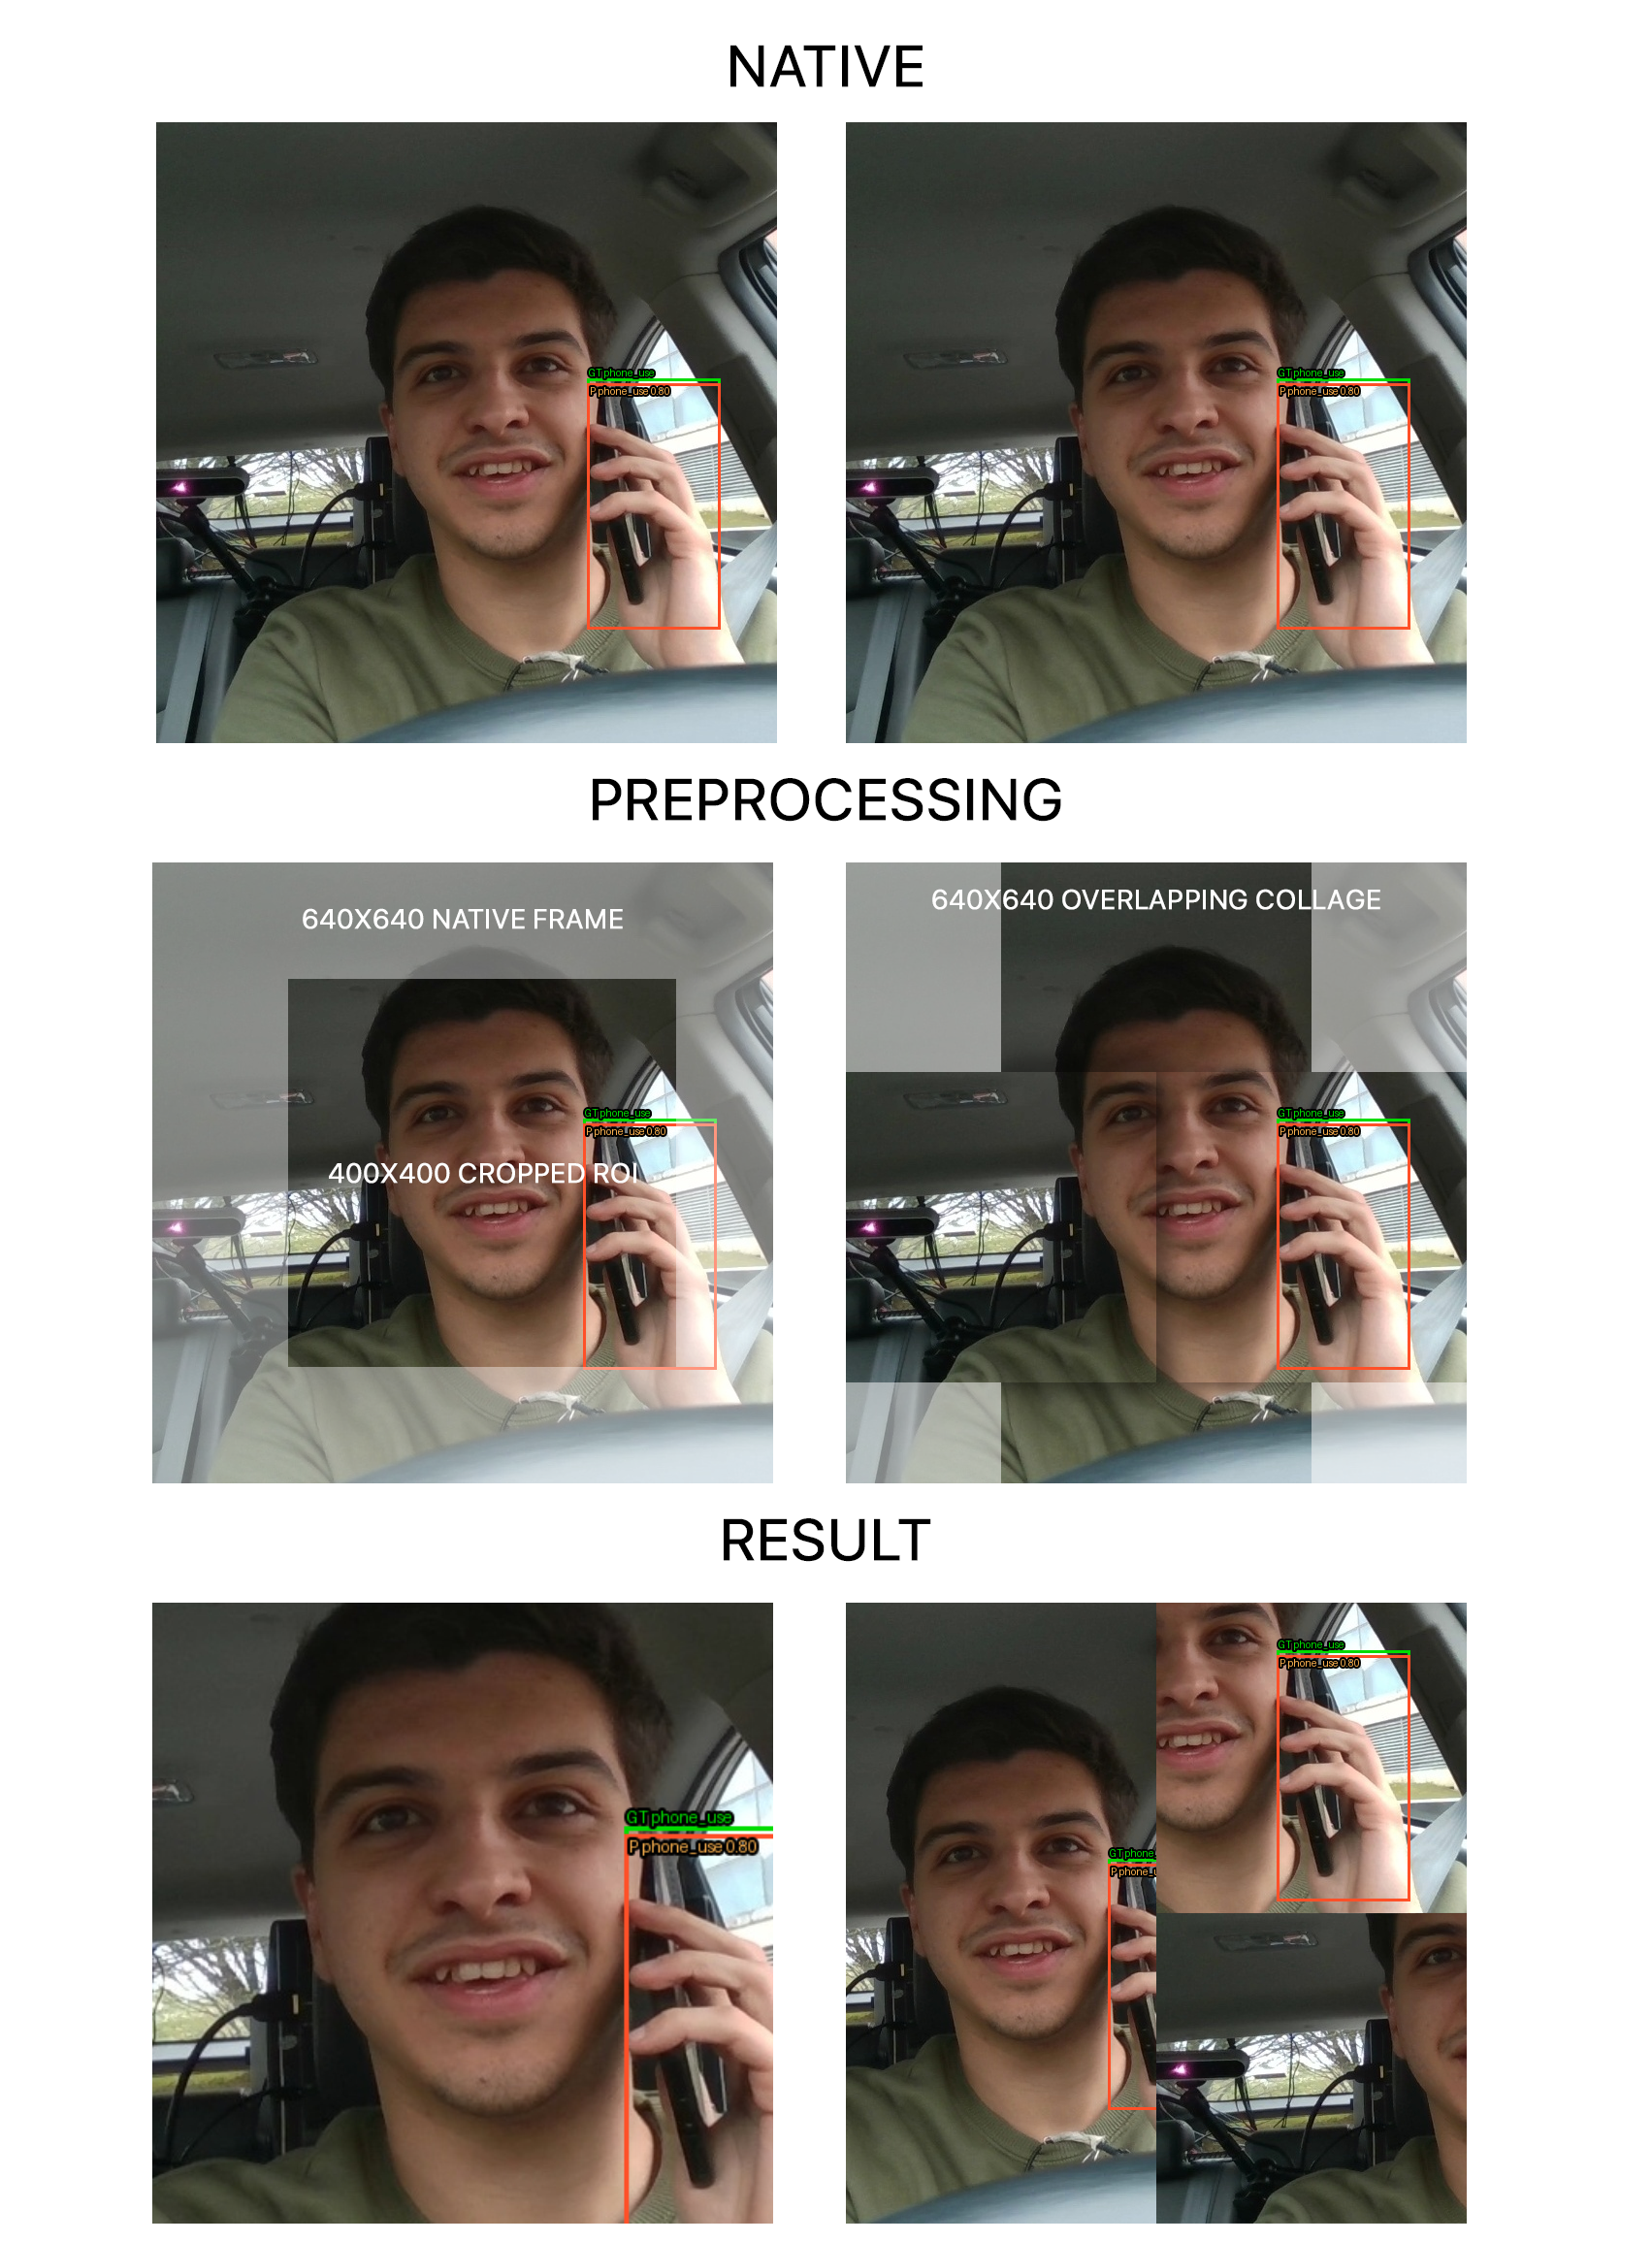
\includegraphics[width=\linewidth]{input_methods.png}
    \caption{Native frames and the output of each input method}
    \label{fig:preprocessing_comparison}
\end{figure}

\subsection{Joint Co-Design}
\label{sec:codesign}
Phase~III evaluates the full grid of 24 INT8 candidates: the three input methods at 320 and 160 pixels, each at 0\%, 30\%, 50\%, and 70\% sparsity. Each candidate starts from the Phase~II checkpoint trained on its input, is pruned as in Section~\ref{sec:pruning}, fine-tuned for up to 50 epochs with a patience of 10, and quantized. Fine-tuning is shorter than in Phase~I because the source model has already converged on the same input. The selection rule (\ref{eq:selection}) picks the candidate on validation data, and test results are reported once. Because validation is small, we also rank all candidates by compute, then memory, and recommend the first whose mean test macro-recall holds the floor in (\ref{eq:floor}). Its paired difference from the baseline, $\Delta R$, and the clip-bootstrap interval are reported with it.


\section{Results and Discussion}
\label{sec:results}

\subsection{Phase I: Model-Side Optimization}

\begin{table*}[!t]
\renewcommand{\arraystretch}{0.85}
\caption{FP32 pruning results on the test set at $\tau=0.5$}
\label{tab:pruning_fixed_tau}
\centering
\scriptsize
\setlength{\tabcolsep}{2.6pt}
\begin{tabular}{@{}lrrrccccccrc@{}}
\toprule
 & \multicolumn{3}{c}{Cost} & & \multicolumn{4}{c}{Class recall (\%)} & & & \\
\cmidrule(lr){2-4}\cmidrule(lr){6-9}
Sparsity & Params (M) & GFLOPs & Size (MB) & $P$ (\%) & Yawning & Hand-mouth & Drinking & Phone use & $R$ (\%) & $\text{Eff}_{\text{FLOPs}}$ & Safe \\
\midrule
\multicolumn{11}{l}{\textit{YOLO11n}} \\
Base & 2.59 & 6.50 & 10.12 & $85.2\pm4.6$ & $80.8\pm1.7$ & $92.9\pm3.6$ & $89.3\pm1.8$ & $82.6\pm1.5$ & $86.4\pm1.3$ & 13.3 & \checkmark \\
10\% & 2.24 & 5.63 & 8.79 & $87.4\pm2.6$ & $80.8\pm6.3$ & $90.5\pm4.1$ & $94.0\pm4.1$ & $79.9\pm3.4$ & $86.3\pm3.7$ & 15.3 & \checkmark \\
20\% & 1.94 & 4.92 & 7.66 & $86.1\pm1.7$ & $83.8\pm7.6$ & $95.2\pm2.1$ & $90.5\pm4.1$ & $82.4\pm1.4$ & $88.0\pm2.9$ & 17.9 & \checkmark \\
30\% & 1.67 & 4.30 & 6.61 & $86.5\pm2.4$ & $84.8\pm8.0$ & $92.9\pm0.0$ & $90.5\pm2.7$ & $80.7\pm2.7$ & $87.2\pm2.1$ & 20.3 & \checkmark \\
40\% & 1.43 & 3.74 & 5.70 & $86.5\pm1.1$ & $76.8\pm6.3$ & $90.5\pm5.5$ & $89.3\pm3.1$ & $81.2\pm1.2$ & $84.4\pm2.3$ & 22.6 & \checkmark \\
50\% & 1.23 & 3.30 & 4.94 & $85.4\pm4.0$ & $78.8\pm5.2$ & $92.9\pm3.6$ & $89.3\pm0.0$ & $81.5\pm0.9$ & $85.6\pm2.3$ & 25.9 & \checkmark \\
60\% & 1.04 & 2.84 & 4.22 & $84.5\pm2.0$ & $85.9\pm7.0$ & $92.9\pm6.2$ & $91.1\pm4.7$ & $82.5\pm1.2$ & $88.1\pm1.2$ & 31.0 & \checkmark \\
70\% & 0.89 & 2.50 & 3.65 & $84.0\pm6.1$ & $79.8\pm6.3$ & $89.3\pm3.6$ & $89.9\pm2.7$ & $83.4\pm1.6$ & $85.6\pm1.4$ & 34.2 & \checkmark \\
80\% & 0.77 & 2.24 & 3.17 & $82.9\pm2.7$ & $61.6\pm9.3$ & $85.7\pm6.2$ & $88.1\pm1.0$ & $83.9\pm3.3$ & $79.8\pm1.8$ & 35.6 & $\times$ \\
90\% & 0.68 & 2.06 & 2.83 & $83.4\pm2.8$ & $16.2\pm1.7$ & $78.6\pm6.2$ & $78.6\pm3.1$ & $75.8\pm1.9$ & $62.3\pm1.7$ & 30.2 & $\times$ \\
\midrule
\multicolumn{11}{l}{\textit{YOLO26n}} \\
Base & 2.51 & 5.90 & 9.34 & $88.5\pm1.1$ & $83.8\pm6.3$ & $95.2\pm2.1$ & $93.5\pm2.1$ & $83.5\pm1.2$ & $89.0\pm1.3$ & 15.1 & \checkmark \\
10\% & 2.18 & 5.03 & 8.12 & $89.7\pm1.8$ & $72.7\pm10.9$ & $92.9\pm0.0$ & $92.3\pm2.7$ & $81.8\pm1.1$ & $84.9\pm3.0$ & 16.9 & \checkmark \\
20\% & 1.91 & 4.33 & 7.08 & $88.0\pm1.4$ & $75.8\pm3.0$ & $92.9\pm3.6$ & $92.3\pm3.7$ & $85.1\pm1.2$ & $86.5\pm2.5$ & 20.0 & \checkmark \\
30\% & 1.66 & 3.72 & 6.11 & $89.7\pm2.9$ & $76.8\pm4.6$ & $90.5\pm2.1$ & $92.9\pm0.0$ & $79.3\pm3.1$ & $84.9\pm1.9$ & 22.8 & \checkmark \\
40\% & 1.43 & 3.16 & 5.27 & $87.3\pm2.3$ & $76.8\pm4.6$ & $91.7\pm5.5$ & $92.3\pm5.5$ & $80.8\pm2.8$ & $85.4\pm4.2$ & 27.0 & \checkmark \\
50\% & 1.25 & 2.73 & 4.56 & $88.9\pm1.6$ & $79.8\pm6.3$ & $96.4\pm0.0$ & $89.9\pm5.5$ & $82.4\pm1.8$ & $87.1\pm1.5$ & 32.0 & \checkmark \\
60\% & 1.07 & 2.26 & 3.86 & $87.7\pm3.7$ & $70.7\pm7.6$ & $92.9\pm3.6$ & $89.9\pm5.5$ & $82.8\pm3.7$ & $84.1\pm3.9$ & 37.1 & \checkmark \\
70\% & 0.92 & 1.93 & 3.32 & $88.1\pm3.0$ & $65.7\pm3.5$ & $84.5\pm5.5$ & $86.3\pm2.1$ & $86.0\pm1.5$ & $80.6\pm0.7$ & 41.9 & $\times$ \\
80\% & 0.80 & 1.67 & 2.85 & $85.8\pm1.6$ & $63.6\pm10.9$ & $82.1\pm3.6$ & $86.3\pm2.7$ & $84.1\pm1.6$ & $79.0\pm1.9$ & 47.4 & $\times$ \\
90\% & 0.71 & 1.48 & 2.50 & $86.2\pm7.6$ & $25.3\pm25.4$ & $71.4\pm15.6$ & $79.2\pm5.7$ & $77.5\pm6.6$ & $63.3\pm5.5$ & 42.7 & $\times$ \\
\bottomrule
\end{tabular}
\end{table*}


\begin{figure}[!t]
\centering
\definecolor{dmsblue}{HTML}{2A78D6}
\definecolor{dmsorange}{HTML}{EB6834}
\definecolor{dmsaqua}{HTML}{1BAF7A}
\definecolor{dmsink}{HTML}{52514E}
\begin{tikzpicture}
\begin{axis}[width=0.95\columnwidth, height=5.0cm, grid=major, grid style={line width=.2pt, draw=gray!30},
  tick label style={font=\scriptsize}, label style={font=\small},
  xlabel={Target sparsity (\%)}, ylabel={$\text{Eff}_{\text{FLOPs}}$},
  xmin=-3, xmax=93, ymin=0, xtick={0,10,...,90},
  legend pos=north west, legend columns=2, legend cell align=left,
  legend style={font=\scriptsize, draw=gray!50}]
\addplot[color=dmsblue, mark=*, mark size=1.5pt, line width=0.9pt] coordinates {(0,13.28) (10,15.33) (20,17.88) (30,20.29) (40,22.59) (50,25.94) (60,31.01) (70,34.21) (80,35.59) (90,30.20)};
\addlegendentry{YOLO11n}
\addplot[color=dmsblue, dashed, line width=0.8pt, mark=none] coordinates {(0,12.51) (10,14.45) (20,16.54) (30,18.93) (40,21.78) (50,24.66) (60,28.66) (70,32.53) (80,36.28) (90,39.46)};
\addlegendentry{YOLO11n limit}
\addplot[color=dmsorange, mark=triangle*, mark size=1.5pt, line width=0.9pt] coordinates {(0,15.09) (10,16.88) (20,20.00) (30,22.83) (40,27.04) (50,31.96) (60,37.13) (70,41.89) (80,47.43) (90,42.73)};
\addlegendentry{YOLO26n}
\addplot[color=dmsorange, dashed, line width=0.8pt, mark=none] coordinates {(0,14.24) (10,16.70) (20,19.42) (30,22.60) (40,26.61) (50,30.82) (60,37.11) (70,43.64) (80,50.40) (90,56.67)};
\addlegendentry{YOLO26n limit}
\end{axis}
\end{tikzpicture}

\caption{FP32 efficiency against target sparsity. A solid line below its dashed limit fails the floor}
\label{fig:pruning_efficiency}
\end{figure}

\begin{table*}[!t]
\renewcommand{\arraystretch}{0.85}
\caption{YOLO11n FP32, INT8 PTQ, and INT8 QAT over three seeds at $\tau=0.5$}
\label{tab:quantization}
\centering
\scriptsize
\setlength{\tabcolsep}{3pt}
\begin{tabular}{@{}rrrc rccrc rccrc@{}}
\toprule
 & & & & \multicolumn{5}{c}{INT8 PTQ} & \multicolumn{5}{c}{INT8 QAT} \\
\cmidrule(lr){5-9}\cmidrule(lr){10-14}
Sparsity (\%) & Param.\ red.\ (\%) & GFLOPs & FP32 $R$ (\%) & MB & $P$ (\%) & $R$ (\%) & $\text{Eff}_{\text{MB}}$ & Safe & MB & $P$ (\%) & $R$ (\%) & $\text{Eff}_{\text{MB}}$ & Safe \\
\midrule
0 & 0.0 & 6.50 & $86.4\pm1.3$ & 3.13 & $85.5\pm5.4$ & $85.6\pm1.3$ & 27.3 & \checkmark & 2.92 & $84.6\pm5.5$ & $86.0\pm1.7$ & 29.5 & \checkmark \\
10 & 13.5 & 5.63 & $86.3\pm3.7$ & 2.81 & $89.0\pm1.8$ & $84.6\pm4.6$ & 30.1 & \checkmark & 2.60 & $87.5\pm3.6$ & $86.3\pm2.9$ & 33.2 & \checkmark \\
20 & 24.9 & 4.92 & $88.0\pm2.9$ & 2.52 & $86.8\pm1.5$ & $87.6\pm1.9$ & 34.7 & \checkmark & 2.31 & $83.8\pm4.0$ & $87.7\pm2.2$ & 37.9 & \checkmark \\
30 & 35.6 & 4.30 & $87.2\pm2.1$ & 2.25 & $87.6\pm2.1$ & $86.9\pm2.1$ & 38.6 & \checkmark & 2.04 & $85.1\pm3.5$ & $86.8\pm2.8$ & 42.5 & \checkmark \\
40 & 44.8 & 3.74 & $84.4\pm2.3$ & 2.02 & $87.1\pm1.5$ & $84.9\pm2.0$ & 42.0 & \checkmark & 1.81 & $87.1\pm3.3$ & $84.0\pm4.9$ & 46.3 & \checkmark \\
50 & 52.5 & 3.30 & $85.6\pm2.3$ & 1.82 & $85.8\pm4.6$ & $85.0\pm2.8$ & 46.7 & \checkmark & 1.62 & $85.2\pm2.3$ & $87.6\pm1.9$ & 54.0 & \checkmark \\
60 & 59.8 & 2.84 & $88.1\pm1.2$ & 1.63 & $84.1\pm1.1$ & $87.7\pm2.3$ & 53.7 & \checkmark & 1.44 & $84.1\pm3.1$ & $86.9\pm0.7$ & 60.5 & \checkmark \\
70 & 65.6 & 2.50 & $85.6\pm1.4$ & 1.48 & $84.2\pm7.1$ & $84.3\pm1.2$ & 56.8 & \checkmark & 1.29 & $83.2\pm5.8$ & $84.8\pm3.0$ & 65.7 & \checkmark \\
80 & 70.4 & 2.24 & $79.8\pm1.8$ & 1.36 & $82.9\pm2.2$ & $78.9\pm1.9$ & 58.0 & $\times$ & 1.17 & $83.7\pm1.7$ & $80.2\pm1.0$ & 68.6 & $\times$ \\
90 & 73.9 & 2.06 & $62.3\pm1.7$ & 1.27 & $80.2\pm8.0$ & $62.0\pm2.2$ & 48.9 & $\times$ & 1.08 & $78.2\pm1.2$ & $61.2\pm0.5$ & 56.7 & $\times$ \\
\bottomrule
\end{tabular}
\end{table*}


\begin{figure}[!t]
\centering
\definecolor{dmsblue}{HTML}{2A78D6}
\definecolor{dmsorange}{HTML}{EB6834}
\definecolor{dmsaqua}{HTML}{1BAF7A}
\definecolor{dmsink}{HTML}{52514E}
\begin{tikzpicture}
\begin{axis}[width=0.95\columnwidth, height=5.0cm, grid=major, grid style={line width=.2pt, draw=gray!30},
  tick label style={font=\scriptsize}, label style={font=\small},
  xlabel={Target sparsity (\%)}, ylabel={Macro-recall (\%)},
  xmin=-3, xmax=93, ymin=0, ymax=100, xtick={0,10,...,90},
  legend pos=south west, legend cell align=left, legend style={font=\scriptsize, draw=gray!50},
  error bars/error bar style={line width=0.5pt, solid},
  error bars/error mark options={line width=0.5pt, mark size=1.2pt, rotate=90}]
\addplot[color=dmsblue, mark=*, mark size=1.5pt, line width=0.9pt, error bars/.cd, y dir=both, y explicit] coordinates {(0,86.38) +- (0,1.31) (10,86.32) +- (0,3.67) (20,88.00) +- (0,2.91) (30,87.22) +- (0,2.13) (40,84.42) +- (0,2.29) (50,85.60) +- (0,2.33) (60,88.07) +- (0,1.22) (70,85.60) +- (0,1.39) (80,79.83) +- (0,1.76) (90,62.27) +- (0,1.66)};
\addlegendentry{FP32}
\addplot[color=dmsorange, mark=square*, mark size=1.5pt, line width=0.9pt, error bars/.cd, y dir=both, y explicit] coordinates {(0,85.60) +- (0,1.35) (10,84.63) +- (0,4.63) (20,87.57) +- (0,1.87) (30,86.94) +- (0,2.13) (40,84.87) +- (0,1.99) (50,85.03) +- (0,2.79) (60,87.67) +- (0,2.32) (70,84.34) +- (0,1.23) (80,78.89) +- (0,1.93) (90,61.96) +- (0,2.25)};
\addlegendentry{INT8 PTQ}
\addplot[color=dmsaqua, mark=triangle*, mark size=1.5pt, line width=0.9pt, error bars/.cd, y dir=both, y explicit] coordinates {(0,85.99) +- (0,1.71) (10,86.34) +- (0,2.94) (20,87.69) +- (0,2.17) (30,86.82) +- (0,2.82) (40,84.02) +- (0,4.94) (50,87.63) +- (0,1.86) (60,86.88) +- (0,0.72) (70,84.78) +- (0,3.04) (80,80.20) +- (0,0.99) (90,61.22) +- (0,0.50)};
\addlegendentry{INT8 QAT}
\end{axis}
\end{tikzpicture}

\caption{YOLO11n macro-recall against target sparsity (mean $\pm$ SD, three seeds)}
\label{fig:quant_macro_recall}
\end{figure}

Tables~\ref{tab:pruning_fixed_tau} and~\ref{tab:quantization} and Figs.~\ref{fig:pruning_efficiency} and~\ref{fig:quant_macro_recall} report Phase~I. Four findings stand out.
\begin{itemize}
\item \emph{Pruning headroom.} YOLO11n holds its 81.4\% floor up to 70\% sparsity ($85.6\pm1.4\%$ against $86.4\pm1.3\%$), then falls to 79.8\% at 80\% and 62.3\% at 90\%. YOLO26n starts higher under the pinned toolchain ($89.0\pm1.3\%$, floor 84.0\%) and holds the floor up to 60\% sparsity ($84.1\pm3.9\%$).
\item \emph{Class sensitivity.} Yawning, the smallest object, fails first. YOLO11n yawning recall falls from 80.8\% at baseline to 61.6\% at 80\% sparsity and 16.2\% at 90\%. Macro-precision stays between 82.9\% and 87.4\%, so pruning costs recall rather than precision.
\item \emph{Cost.} At 70\% sparsity YOLO11n has 0.89M parameters, 2.50~GFLOPs, and a 3.65~MB FP32 ONNX file, against 2.59M, 6.50~GFLOPs, and 10.12~MB. Parameters fall by only 65.6\% because the excluded head grows from 16.7\% to 48.4\% of the remaining weights.
\item \emph{Quantization.} PTQ and QAT stay within 2.1~pp of FP32 at every sparsity up to 70\%, with seed SD at most 4.9~pp. At 70\% sparsity, PTQ gives $84.3\pm1.2\%$ in 1.48~MB and QAT gives $84.8\pm3.0\%$ in 1.29~MB. Both store the same 0.83~MB of INT8 weights. The PTQ file is larger because it quantizes every activation (795 quantize and dequantize nodes against 273), while QAT quantizes only convolution inputs. Both INT8 formats keep FP32 precision. Both fail at 80\%, as FP32 does.
\end{itemize}
INT8 recall was stable only after a change of calibration. With plain MinMax ranges, PTQ recall varied by up to 32~pp between seeds of one configuration, and one seed reached 27.2\% at 80\% sparsity. Ranking survived: mAP@0.5 stayed at 0.87, and the confidences of the true class kept a 0.97 correlation with FP32 but halved in value. One rare outlier activation had set a range 12 times wider than typical, so the fixed threshold rejected correct detections. A moving average of per-frame extremes restored that seed to 77.5\%. Class-balanced calibration frames did not help (30.4\%). QAT also freezes its ranges after a short calibration, but it then trains the weights under those ranges, so the network adapts to any clipping. The earlier submission also quantized the class-logit outputs of the head, whose 40 to 150 unit range gives a step of 0.15 to 0.59 logit near the threshold. We keep those layers in floating point.

\subsection{Phase II: Input-Side Optimization}

\begin{table*}[!t]
\renewcommand{\arraystretch}{0.9}
\caption{FP32 YOLO11n by input method and resolution at $\tau=0.5$}
\label{tab:accuracy}
\centering
\footnotesize
\setlength{\tabcolsep}{5pt}
\begin{tabular}{@{}rrccc rrrc@{}}
\toprule
Input (px) & GFLOPs & $P$ (\%) & $R$ (\%) & $F1$ (\%) & mAP@0.5 & mAP@0.5:0.95 & $R$ strict\textsuperscript{a} (\%) & Safe \\
\midrule
\multicolumn{9}{l}{\textit{Resize}} \\
640 & 6.50 & $84.9\pm4.0$ & $87.4\pm2.6$ & $84.6\pm2.0$ & 92.5 & 55.6 & 87.4 & \checkmark \\
320 & 1.61 & $87.3\pm1.4$ & $88.3\pm1.2$ & $87.4\pm0.9$ & 93.3 & 58.8 & 88.3 & \checkmark \\
160 & 0.40 & $88.3\pm1.5$ & $80.7\pm1.6$ & $83.1\pm0.8$ & 90.8 & 54.3 & 80.7 & $\times$ \\
80 & 0.14 & $87.3\pm0.6$ & $72.6\pm1.7$ & $77.1\pm1.3$ & 84.3 & 47.3 & 72.6 & $\times$ \\
\midrule
\multicolumn{9}{l}{\textit{Crop}} \\
640 & 6.50 & $87.1\pm1.7$ & $81.5\pm2.3$ & $83.2\pm1.0$ & 87.8 & 58.8 & 72.6 & \checkmark \\
320 & 1.61 & $87.5\pm2.5$ & $84.7\pm0.8$ & $85.4\pm1.4$ & 89.0 & 61.4 & 75.8 & \checkmark \\
160 & 0.40 & $87.8\pm1.0$ & $82.3\pm3.1$ & $84.2\pm1.7$ & 86.6 & 58.2 & 73.5 & \checkmark \\
80 & 0.14 & $86.3\pm4.6$ & $75.7\pm2.6$ & $79.0\pm2.1$ & 84.5 & 53.2 & 67.0 & $\times$ \\
\midrule
\multicolumn{9}{l}{\textit{Collage}} \\
640 & 6.50 & $86.9\pm2.4$ & $90.5\pm2.2$ & $87.9\pm1.2$ & 92.3 & 66.8 & 89.0 & \checkmark \\
320 & 1.61 & $86.6\pm0.8$ & $93.2\pm0.7$ & $89.2\pm0.7$ & 92.6 & 67.9 & 91.1 & \checkmark \\
160 & 0.40 & $82.5\pm1.7$ & $88.7\pm1.8$ & $84.8\pm1.5$ & 87.1 & 59.8 & 87.1 & \checkmark \\
80 & 0.14 & $82.9\pm2.8$ & $75.3\pm3.0$ & $76.7\pm1.4$ & 80.0 & 49.9 & 73.5 & $\times$ \\
\bottomrule
\multicolumn{9}{l}{\textsuperscript{a}A box counts only if at least 50\% of it stays visible.} \\
\end{tabular}
\end{table*}


\begin{figure}[!t]
\centering
\definecolor{dmsblue}{HTML}{2A78D6}
\definecolor{dmsorange}{HTML}{EB6834}
\definecolor{dmsaqua}{HTML}{1BAF7A}
\definecolor{dmsink}{HTML}{52514E}
\begin{tikzpicture}
\begin{axis}[width=0.95\columnwidth, height=5.0cm, xmode=log, log basis x=10, grid=major,
  grid style={line width=.2pt, draw=gray!30}, tick label style={font=\scriptsize}, label style={font=\small},
  xlabel={GFLOPs}, ylabel={Macro-recall (\%)}, xmin=0.1, xmax=10, ymin=60, ymax=100,
  legend pos=south east, legend cell align=left, legend style={font=\scriptsize, draw=gray!50}]
\addplot[only marks, color=dmsblue, mark=*, mark size=2.2pt] coordinates {(0.144962,72.63) (0.402826,80.66) (1.61418,88.33) (6.50281,87.43)};
\addlegendentry{Resize}
\addplot[only marks, color=dmsorange, mark=square*, mark size=2.2pt] coordinates {(0.144962,75.72) (0.402826,82.35) (1.61418,84.72) (6.50281,81.51)};
\addlegendentry{Crop}
\addplot[only marks, color=dmsaqua, mark=triangle*, mark size=2.2pt] coordinates {(0.144962,75.33) (0.402826,88.68) (1.61418,93.21) (6.50281,90.47)};
\addlegendentry{Collage}
\addplot[color=dmsink, dashed, line width=0.8pt, forget plot] coordinates {(0.1,81.38) (10,81.38)};
\end{axis}
\end{tikzpicture}

\caption{FP32 macro-recall against compute for each input method. The dashed line is the floor}
\label{fig:input_methods}
\end{figure}

Table~\ref{tab:accuracy} and Fig.~\ref{fig:input_methods} report Phase~II. Four findings stand out.
\begin{itemize}
\item \emph{Resolution headroom.} Resizing the full frame holds recall down to 320 pixels (88.3\% at 1.61~GFLOPs). At 160 pixels it fails the floor (80.7\%) because yawning recall falls to 56.6\%.
\item \emph{Crop.} Magnifying the face lifts yawning recall at 160 pixels from 56.6\% to 87.9\%. The window cuts peripheral objects, though: phone-use recall stays near 70\% at every resolution. When a box must stay at least half visible to count, the crop falls below the floor at every resolution.
\item \emph{Collage.} The collage gives the highest recall at every resolution from 640 to 160 pixels: 90.5\%, 93.2\%, and 88.7\%, with F1 of 0.892 at 320 pixels. It holds 87.1\% to 91.1\% under the stricter visibility rule. The overlapping tiles show the face and hand zones twice, which helps most for yawning (96.0\% at 320 pixels against 87.9\% for resize). The first submission scored each tile fragment as a separate object, which hid this result.
\item \emph{Lower limit.} No method holds the floor at 80 pixels.
\end{itemize}

\subsection{Phase III: System Co-Design}

\definecolor{dmsblue}{HTML}{2A78D6}
\definecolor{dmsorange}{HTML}{EB6834}
\definecolor{dmsaqua}{HTML}{1BAF7A}
\definecolor{dmsink}{HTML}{52514E}
\begin{table*}[!t]
\renewcommand{\arraystretch}{0.95}
\caption{Test macro-recall (\%) of INT8 PTQ models across input, resolution, and sparsity}
\label{tab:codesign_study}
\centering
\footnotesize
\setlength{\tabcolsep}{6pt}
\begin{tabular}{@{}llcccc@{}}
\toprule
 & & \multicolumn{4}{c}{Sparsity} \\
\cmidrule(l){3-6}
 & & 0\% & 30\% & 50\% & 70\% \\
\midrule
\multicolumn{2}{@{}l}{\textit{320 px}: GFLOPs / MB} & 1.61 / 3.01 & 1.06 / 2.13 & 0.81 / 1.70 & 0.61 / 1.36 \\
\cmidrule(l){3-6}
 & Resize & 86.1 $\pm$ 1.0 \checkmark & 79.6 $\pm$ 6.7 $\times$ & 78.7 $\pm$ 4.1 $\times$ & 72.1 $\pm$ 3.7 $\times$ \\
 & Crop & 83.8 $\pm$ 1.7 \checkmark & 81.5 $\pm$ 3.6 \checkmark & 77.1 $\pm$ 7.1 $\times$ & 65.4 $\pm$ 5.3 $\times$ \\
 & Collage & 92.9 $\pm$ 0.2 \checkmark & 89.8 $\pm$ 1.5 \checkmark & 89.8 $\pm$ 0.5 \checkmark & 78.0 $\pm$ 0.9 $\times$ \\
\midrule
\multicolumn{2}{@{}l}{\textit{160 px}: GFLOPs / MB} & 0.40 / 2.98 & 0.27 / 2.10 & 0.20 / 1.67 & 0.15 / 1.33 \\
\cmidrule(l){3-6}
 & Resize & 70.4 $\pm$ 1.8 $\times$ & 65.7 $\pm$ 3.5 $\times$ & 63.8 $\pm$ 0.5 $\times$ & 43.3 $\pm$ 4.3 $\times$ \\
 & Crop & 78.7 $\pm$ 3.3 $\times$ & 72.5 $\pm$ 0.7 $\times$ & 67.7 $\pm$ 8.4 $\times$ & 48.2 $\pm$ 6.7 $\times$ \\
 & Collage & 83.8 $\pm$ 4.8 \checkmark & \cellcolor{dmsaqua!22}\textbf{81.5 $\pm$ 4.3 \checkmark} & 73.8 $\pm$ 4.8 $\times$\textsuperscript{S} & 46.2 $\pm$ 2.5 $\times$ \\
\midrule
\multicolumn{2}{@{}l}{Baseline, 640 px, FP32} & \multicolumn{4}{l}{86.4 $\pm$ 1.3 at 6.50 GFLOPs / 10.12 MB} \\
\bottomrule
\end{tabular}

\smallskip
{\scriptsize Mean $\pm$ SD over three seeds. \checkmark: holds the 81.4\% floor. Shaded: the cheapest configuration that holds it. S: selected on validation by (\ref{eq:selection}).}
\end{table*}

\begin{table}[t]
\caption{Test recall (\%) with clip-bootstrap 95\% intervals}
\label{tab:uncertainty}
\centering
\footnotesize
\setlength{\tabcolsep}{2.5pt}
\begin{tabular}{@{}lccc@{}}
\toprule
\textbf{Class} & \textbf{Baseline} & \textbf{Selected (S)} & \textbf{Recommended (R)} \\
\midrule
Yawning & 80.8 (64--94) & 31.3 (21--47) & 94.9 (82--99) \\
Hand-over-mouth & 92.9 (67--100) & 90.5 (71--98) & 96.4 (80--100) \\
Drinking & 89.3 (79--100) & 89.9 (85--95) & 97.6 (96--100) \\
Phone use & 82.6 (50--99) & 83.4 (50--100) & 82.6 (47--100) \\
\midrule
Macro & 86.4 (73--95) & 73.8 (63--81) & 92.9 (82--98) \\
\bottomrule
\end{tabular}
\end{table}


\begin{figure}[!t]
\centering
\definecolor{dmsblue}{HTML}{2A78D6}
\definecolor{dmsorange}{HTML}{EB6834}
\definecolor{dmsaqua}{HTML}{1BAF7A}
\definecolor{dmsink}{HTML}{52514E}
\begin{tikzpicture}
\begin{axis}[width=0.95\columnwidth, height=5.2cm, xmode=log, log basis x=10, grid=major,
  grid style={line width=.2pt, draw=gray!30}, tick label style={font=\scriptsize}, label style={font=\small},
  xlabel={GFLOPs}, ylabel={Test macro-recall (\%)}, xmin=0.1, xmax=10, ymin=40, ymax=100,
  legend pos=south east, legend cell align=left, legend style={font=\scriptsize, draw=gray!50},
  error bars/error bar style={line width=0.5pt, solid},
  error bars/error mark options={line width=0.5pt, mark size=1.2pt, rotate=90}]
\addplot[only marks, color=dmsblue, mark=*, mark size=2.2pt, error bars/.cd, y dir=both, y explicit] coordinates {(1.614,86.11) +- (0,0.95) (0.614,72.15) +- (0,3.67)};
\addlegendentry{Resize}
\addplot[only marks, color=dmsorange, mark=square*, mark size=2.2pt, error bars/.cd, y dir=both, y explicit] coordinates {(0.403,78.74) +- (0,3.35) (0.265,72.51) +- (0,0.72) (1.614,83.85) +- (0,1.69) (0.814,77.12) +- (0,7.07) (0.614,65.35) +- (0,5.26)};
\addlegendentry{Crop}
\addplot[only marks, color=dmsaqua, mark=triangle*, mark size=2.2pt, error bars/.cd, y dir=both, y explicit] coordinates {(0.403,83.84) +- (0,4.77) (0.265,81.53) +- (0,4.32) (0.203,73.76) +- (0,4.81) (0.153,46.23) +- (0,2.51) (1.614,92.89) +- (0,0.19) (0.614,78.02) +- (0,0.89)};
\addlegendentry{Collage}
\addplot[only marks, color=black, mark=diamond*, mark size=2.6pt] coordinates {(6.503,86.38)};
\addlegendentry{Baseline FP32}
\addplot[color=dmsink, dashed, line width=0.8pt, forget plot] coordinates {(0.1,81.38) (10,81.38)};
\end{axis}
\end{tikzpicture}

\caption{Test macro-recall of every INT8 candidate against compute, with solid lines at 320 pixels and dashed lines at 160 pixels. The shaded band clears the floor, hollow markers fail it, and the ringed point is the recommended configuration}
\label{fig:codesign}
\end{figure}

Table~\ref{tab:codesign_study}, Table~\ref{tab:uncertainty}, and Fig.~\ref{fig:codesign} report Phase~III. Four findings stand out.
\begin{itemize}
\item \emph{Pruning at reduced input.} Pruning hurts more when the input is small. At 320 pixels the collage holds the floor up to 50\% sparsity (89.8\%), the crop up to 30\% (81.5\%), and resize only unpruned (79.6\% at 30\%). At 70\% sparsity all three methods fail at 320 pixels (65.4\% to 78.0\%), although the same sparsity holds the floor at 640 pixels. At 160 pixels resize and crop fail even unpruned (70.4\% and 78.7\%). On the 160-pixel collage, 30\% sparsity still holds (81.5\%), 50\% does not (73.8\%), and 70\% collapses (46.2\%).
\item \emph{Validation does not transfer.} The rule in (\ref{eq:selection}) selects the 160-pixel collage with 50\% sparsity, at 0.20~GFLOPs, which is 1.3~pp above the baseline on validation. On the test drivers it falls 12.6~pp below the baseline because yawning recall drops to 31.3\% (95\% interval 21\% to 47\%). Three validation subjects with about 30 frames per rare class cannot certify a configuration that changes both input scale and network width.
\item \emph{Recommended configuration.} Table~\ref{tab:codesign_study} ranks every candidate by compute, then memory, and Fig.~\ref{fig:codesign} shows the same ranking against the floor. Every candidate cheaper than 0.27~GFLOPs fails. The first that holds the floor is the 160-pixel collage with 30\% sparsity and INT8 PTQ: $81.5\pm4.3\%$ macro-recall at 0.27~GFLOPs and 2.10~MB, which is $24.5\times$ less compute and $4.8\times$ less storage than the FP32 ONNX baseline. It is the least costly configuration this study supports, not a comfortable one: it clears the floor by 0.1~pp, its 95\% interval spans 69.5\% to 88.5\%, and yawning recall falls to 49.5\%.
\item \emph{More recall for more compute.} The unpruned 160-pixel collage with INT8 holds 83.8\% at 0.40~GFLOPs and 2.98~MB. Pruning the 320-pixel collage to 50\% keeps $89.8\pm0.5\%$ at 0.81~GFLOPs and 1.70~MB ($8.0\times$ less compute), and stays above the floor under the stricter visibility rule (86.8\%) and the tuned threshold (86.7\%). The 320-pixel collage with INT8 gives the highest recall, $92.9\pm0.2\%$ at 1.61~GFLOPs and 3.01~MB ($4.0\times$ less compute), 6.5~pp above the baseline (95\% interval 0.9 to 13.6~pp), with every class at 82.6\% or more. It is the choice when the margin matters more than the last factor of compute.
\end{itemize}

Two further checks qualify these results. The recommended configuration falls just below the floor under the stricter visibility rule (79.3\%) and under a validation-tuned threshold (80.0\%), so its pass at $\tau=0.5$ is narrow. The 320-pixel collage keeps 91.1\% and 89.4\% under the same checks, and the selected 50\% configuration fails under both. Because the recommendation uses test results, we report it as a recommendation and not as a validated selection. The two INT8 sizes in the first submission, 1.31 and 1.19~MB for one network, differ only by the anchor tables that a fixed-shape graph stores: 0.128~MB at 640 pixels and 0.032~MB at 320 pixels.

\subsection{Limitations and Future Work}
\label{sec:limitations}
The test set holds three drivers and each rare class comes from five clips, so our intervals are wide, and the failed selection in Phase~III shows that three validation drivers cannot certify a pruned low-resolution model. We did not measure latency, power, or memory on automotive hardware, where INT8 support changes the real gains, and an integer-only accelerator would also have to run the floating-point head outputs. The crop and collage also assume a fixed camera mount. Future work should add drivers and cabins, select configurations with cross-validation over subjects, and measure the recommended pipeline on target hardware.


\section{Conclusion}
This paper asked whether model compression and input preprocessing can be co-designed for edge driver monitoring without violating a safety recall floor. We evaluated structured $\ell_1$-norm pruning with INT8 PTQ and QAT on YOLO11n and YOLO26n, together with resize, crop, and collage inputs from 640 to 80 pixels, under one protocol on the same subject-disjoint frames and boxes. Three conclusions follow. First, the model has real headroom at full resolution, because YOLO11n holds the floor up to 70\% sparsity and INT8 keeps that recall at 1.3 to 1.5~MB once ranges are calibrated with a moving average. Second, the input matters as much as the model, because the overlapping collage gives the highest recall at every resolution down to 160 pixels, while a static crop loses peripheral cues such as phone use. Third, the two levers combine well only in moderation. The cheapest configuration that holds the floor, a 160-pixel collage with 30\% sparsity and INT8, needs $24.5\times$ less compute than the baseline but passes only narrowly, while the 320-pixel collage with INT8 keeps 92.9\% recall at $4.0\times$ less compute. Heavier pruning at reduced input did not transfer from validation to test drivers, so input reshaping and quantization are the safer levers, and on-device tests with more drivers are the next step.


\IEEEtriggeratref{13}
\begin{thebibliography}{00}
\bibitem{b1} J. Guo, W. Ouyang, and D. Xu, ``Multi-dimensional pruning: A unified framework for model compression,'' in \emph{Proc. IEEE/CVF Conf. Comput. Vis. Pattern Recognit. (CVPR)}, 2020, pp. 1508--1517.
\bibitem{b2} A. Vina, ``Pruning and quantization in computer vision: A quick guide,'' Ultralytics Blog, Jul. 11, 2025. Accessed: Sep. 29, 2026. [Online]. Available: \url{https://www.ultralytics.com/blog/pruning-and-quantization-in-computer-vision-a-quick-guide}
\bibitem{b3} Y. He, P. Liu, L. Zhu, and Y. Yang, ``Filter pruning by switching to neighboring CNNs with good attributes,'' \emph{IEEE Trans. Neural Netw. Learn. Syst.}, pp. 1--13, 2022, doi: 10.1109/TNNLS.2022.3149332.
\bibitem{b4} Z. Wang, C. Li, and X. Wang, ``Convolutional neural network pruning with structural redundancy reduction,'' in \emph{Proc. IEEE/CVF Conf. Comput. Vis. Pattern Recognit. (CVPR)}, 2021, pp. 14913--14922.
\bibitem{b5} Z. Li, B. Ni, T. Li, and W. Gao, ``Residual quantization for low bit-width neural networks,'' \emph{IEEE Trans. Multimedia}, vol. 25, pp. 214--227, 2023, doi: 10.1109/TMM.2021.3124095.
\bibitem{b6} S. Li \emph{et al.}, ``Distilling a powerful student model via online knowledge distillation,'' \emph{IEEE Trans. Neural Netw. Learn. Syst.}, pp. 1--10, 2022, doi: 10.1109/TNNLS.2022.3152732.
\bibitem{b8} S. Han, H. Mao, and W. J. Dally, ``Deep compression: Compressing deep neural networks with pruning, trained quantization and Huffman coding,'' in \emph{Proc. Int. Conf. Learn. Represent. (ICLR)}, 2016.
\bibitem{b9} H. Li, A. Kadav, I. Durdanovic, H. Samet, and H. P. Graf, ``Pruning filters for efficient ConvNets,'' in \emph{Proc. Int. Conf. Learn. Represent. (ICLR)}, 2017.
\bibitem{b10} Y. He, X. Zhang, and J. Sun, ``Channel pruning for accelerating very deep neural networks,'' in \emph{Proc. IEEE Int. Conf. Comput. Vis. (ICCV)}, 2017, pp. 1389--1397.
\bibitem{b11} Z. Liu, J. Li, Z. Shen, G. Huang, S. Yan, and C. Zhang, ``Learning efficient convolutional networks through network slimming,'' in \emph{Proc. IEEE Int. Conf. Comput. Vis. (ICCV)}, 2017, pp. 2736--2744.
\bibitem{b12} G. Fang, X. Ma, M. Song, M. B. Mi, and X. Wang, ``DepGraph: Towards any structural pruning,'' in \emph{Proc. IEEE/CVF Conf. Comput. Vis. Pattern Recognit. (CVPR)}, 2023, pp. 16091--16101.
\bibitem{b13} B. Jacob, S. Kligys, B. Chen, M. Zhu, M. Tang, A. Howard, H. Adam, and D. Kalenichenko, ``Quantization and training of neural networks for efficient integer-arithmetic-only inference,'' in \emph{Proc. IEEE/CVF Conf. Comput. Vis. Pattern Recognit. (CVPR)}, 2018, pp. 2704--2713.
\bibitem{b14} R. Krishnamoorthi, ``Quantizing deep convolutional networks for efficient inference: A whitepaper,'' arXiv:1806.08342, 2018.
\bibitem{b15} C.-Y. Wang, A. Bochkovskiy, and H.-Y. M. Liao, ``YOLOv7: Trainable bag-of-freebies sets new state-of-the-art for real-time object detectors,'' in \emph{Proc. IEEE/CVF Conf. Comput. Vis. Pattern Recognit. (CVPR)}, 2023, pp. 7464--7475.
\bibitem{b16} A. Wang, H. Chen, L. Liu, K. Chen, Z. Lin, J. Han, and G. Ding, ``YOLOv10: Real-time end-to-end object detection,'' in \emph{Proc. Adv. Neural Inf. Process. Syst. (NeurIPS)}, vol. 37, 2024.
\bibitem{b17} R. Khanam and M. Hussain, ``YOLOv11: An overview of the key architectural enhancements,'' arXiv:2410.17725, 2024.
\bibitem{b26} R. Sapkota, R. H. Cheppally, A. Sharda, and M. Karkee, ``YOLO26: Key architectural enhancements and performance benchmarking for real-time object detection,'' arXiv:2509.25164, 2025.
\bibitem{b18} F. O. Unel, B. O. Ozkalayci, and C. Cigla, ``The power of tiling for small object detection,'' in \emph{Proc. IEEE/CVF Conf. Comput. Vis. Pattern Recognit. Workshops (CVPRW)}, 2019, pp. 582--591.
\bibitem{b19} M. Najibi, B. Singh, and L. S. Davis, ``AutoFocus: Efficient multi-scale inference,'' in \emph{Proc. IEEE/CVF Int. Conf. Comput. Vis. (ICCV)}, 2019, pp. 9745--9755.
\bibitem{b20} J. D. Ortega, N. Kose, P. Ca\~{n}as, M.-A. Chao, A. Unnervik, M. Nieto, O. Otaegui, and L. Salgado, ``DMD: A large-scale multi-modal driver monitoring dataset for attention and alertness analysis,'' in \emph{Proc. Eur. Conf. Comput. Vis. Workshops (ECCVW)}, 2020, pp. 387--405.
\bibitem{b21} Y. Abouelnaga, H. M. Eraqi, and M. N. Moustafa, ``Real-time distracted driver posture classification,'' arXiv:1706.09498, 2017.
\bibitem{b22} A. Kashevnik, R. Shchedrin, C. Kaiser, and A. Stocker, ``Driver distraction detection methods: A literature review and framework,'' \emph{IEEE Access}, vol. 9, pp. 60063--60076, 2021.
\bibitem{euroncap2026driver} Euro NCAP, ``Safe Driving: Driver Engagement Protocol,'' Version 1.2, Euro NCAP, Leuven, Belgium, Jul. 2026. [Online]. Available: \url{https://cdn.euroncap.com/cars/assets/Euro_NCAP_Protocol_Safe_Driving_Driver_Engagement_v1_2_ebce03a443.pdf}
\bibitem{isots5283} \textit{Road Vehicles: Driver Readiness and Intervention Management, Part 1: Partial Automation (Level 2)}, ISO/TS 5283-1:2025, International Organization for Standardization, Geneva, Switzerland, Oct. 2025. [Online]. Available: \url{https://www.iso.org/standard/85035.html}
\end{thebibliography}

\end{document}
